%-------------------------------------------------------------------------------
% 请勿删除本注释
% Free Response Question 1
%
% 指引:
% 如在小问之前有通用问题描述,请放置于此
%-------------------------------------------------------------------------------
\begin{figure}[H]
\centering
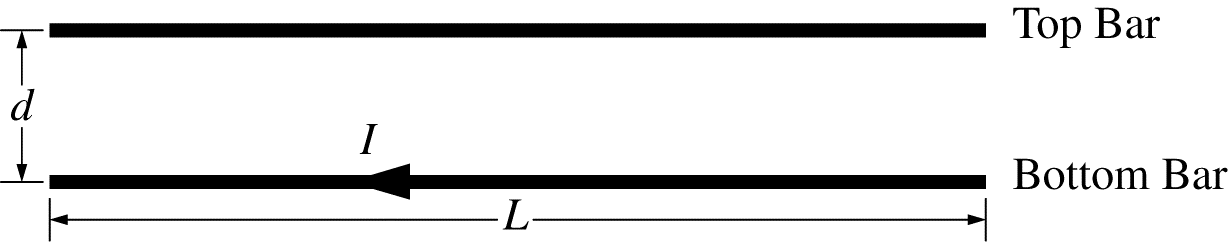
\includegraphics[scale=0.3]{images/img-017-029.png}
\end{figure}


\question
Two metal bars of length $L$ are held a vertical distance $d$ apart $(L>d)$, as shown in the figure above. Each wire carries a current $I$, and the wires repel each other. The current is to the left in the bottom metal bar. % 请删除并替换本行,与上一行 \question 之间不要留空行

\begin{parts}

%-------------------------------------------------------------------------------
% 请勿删除本注释
% Part (a)
%
% 指引:
% 如在小问之前有通用问题描述,请放置于此
%-------------------------------------------------------------------------------

\part
In the figure above, draw an arrow indicating the direction of the current in the top bar. % 请删除并替换本行,与上一行 \part 之间不要留空行

%-------------------------------------------------------------------------------
% 请勿删除本注释
% Part (b)
%
% 指引:
% 如在小问之前有通用问题描述,请放置于此
%-------------------------------------------------------------------------------

\part
In the figure above, use appropriate symbols to indicate the direction of the magnetic field both above and below the bottom bar due to its current $I$. % 请删除并替换本行,与上一行 \part 之间不要留空行

%-------------------------------------------------------------------------------
% 请勿删除本注释
% Part (c)
%
% 指引:
% 如在小问之前有通用问题描述,请放置于此
%-------------------------------------------------------------------------------

\part
Derive an expression for the magnetic force acting on the top bar in terms of $I, L, d$, and fundamental constants, as appropriate. % 请删除并替换本行,与上一行 \part 之间不要留空行

%-------------------------------------------------------------------------------
% 请勿删除本注释
% Part (d)
%
% 指引:
% 如在小问之前有通用问题描述,请放置于此
%-------------------------------------------------------------------------------
The bars are now used in an experiment, as shown in the figure below. The bottom bar is fixed in place. The top bar is suspended from springs (that are not shown), is free to move up and down, and has a pan attached to it for adding small weights. The top bar is originally horizontal and balanced in the equilibrium position as shown. No current is flowing in the bars. Both bars are part of the same closed circuit (the remainder of the circuit is not shown) and connected to a variable power supply. A small object is placed in the pan on the top bar, forcing it down until it comes close to the bottom bar. The current is turned on and increased until it pushes the top bar back to its original equilibrium position. The process is repeated several times with different objects of known mass, and the current is measured with an ammeter each time. The resulting data are given in the table below.


\begin{figure}[H]
\centering
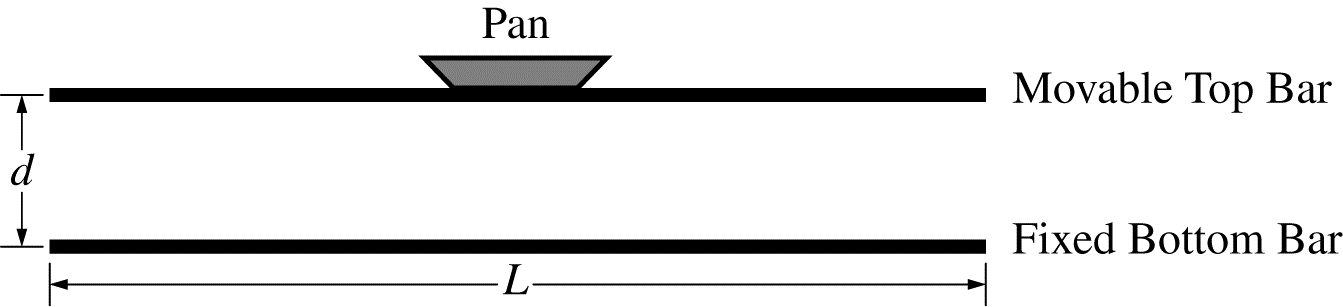
\includegraphics[scale=0.3]{images/img-018-030.png}
\end{figure}


\begin{table}[H]
\centering
\begin{tabular}{|c|c|c|}
\hline Weight of Object in Pan $(\mathrm{N})$ & Current $(\mathrm{A})$ & Current $^{2}\left(\mathrm{~A}^{2}\right)$ \\
\hline $1.00 \times 10^{-4}$ & $5.3$ & $27.9$ \\
\hline $2.00 \times 10^{-4}$ & $7.6$ & $58.4$ \\
\hline $3.00 \times 10^{-4}$ & $9.6$ & $91.4$ \\
\hline $4.00 \times 10^{-4}$ & $11.3$ & 128 \\
\hline $5.00 \times 10^{-4}$ & $12.5$ & 157 \\
\hline
\end{tabular}
\end{table}



\part
Plot the current squared as a function of the weight of the objects on the grid below. Clearly scale and label all axes and include units as appropriate. % 请删除并替换本行,与上一行 \part 之间不要留空行

\begin{figure}[H]
\centering
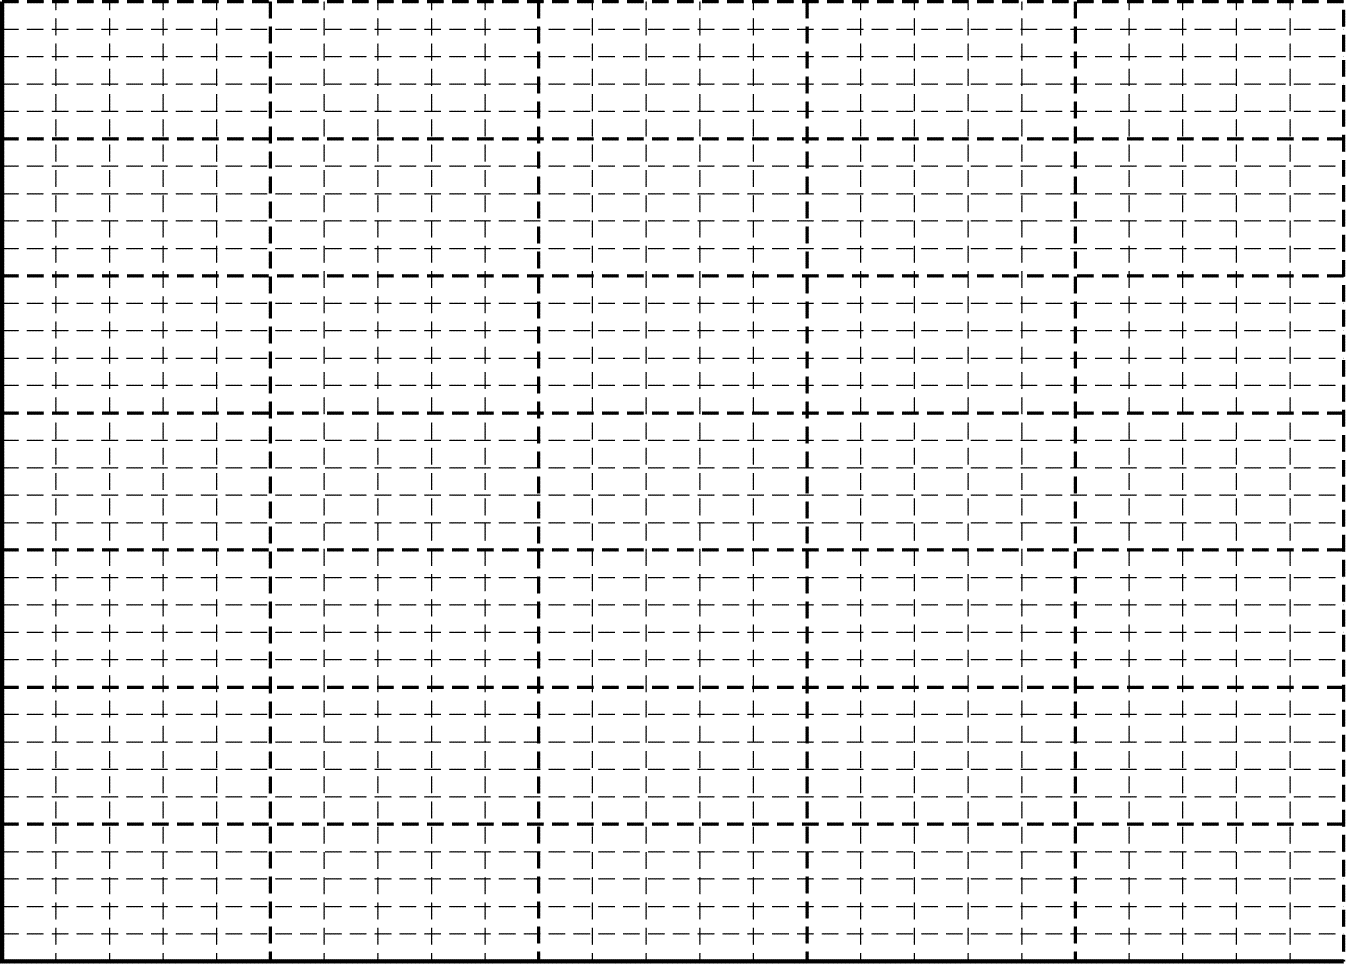
\includegraphics[scale=0.3]{images/img-018-031.png}
\end{figure}


%-------------------------------------------------------------------------------
% 请勿删除本注释
% Part (e)
%
% 指引:
% 如在小问之前有通用问题描述,请放置于此
%-------------------------------------------------------------------------------

\part
Draw a straight line that best represents the data points and write the equation of the line. % 请删除并替换本行,与上一行 \part 之间不要留空行

%-------------------------------------------------------------------------------
% 请勿删除本注释
% Part (f)
%
% 指引:
% 如在小问之前有通用问题描述,请放置于此
%-------------------------------------------------------------------------------

\part
The length of the bars $L$ is $10.2 \mathrm{~cm}$. The center-to-center distance $d$ between the bars is $6.24 \mathrm{~mm}$. Using the equation of the line determined in part (e), calculate a numerical value for the vacuum permeability $\mu_{0}$. % 请删除并替换本行,与上一行 \part 之间不要留空行

\end{parts}


